\chapter{La trave}

%Ci siamo finora occupati separatamente degli aspetti deformativi, di equilibrio e costitutivi, ignorando che, a causa del legame costitutivo a deformazioni corrispondono delle tensioni e viceversa.
 In questo capitolo ci occupiamo di formulare il problema elastico per la trave, tenendo conto di tutti e tre gli ingredienti: cinematici, dinamici e costitutivi. 

\section{Il problema elastico}
In analogia con quanto discusso nel caso dei continui 3D, possiamo formulare il problema elastico nel caso della trave.
% Ci limiteremo a considerare solo il caso piano.

L'obiettivo è determinare lo \textit{stato elastico}, ovvero l'insieme di campi
%\begin{equation}
%\{   \varepsilon, \gamma, \kappa; w, v, \varphi; N, T, M  \}
%\end{equation} 
\begin{equation}
\{\eb, \kb ; \ub, \varthetab ;\fb, \mb;  \}
\end{equation}
di deformazioni, spostamenti e sforzi che siano \textit{congruenti}, ovvero
\begin{equation}\label{eqcongrp}
\eb=\ub'-\varthetab\times \eb_3, \qquad \kb=\varthetab'
%\varepsilon=w', \qquad \gamma=v'+\varphi, \qquad \kappa=\varphi',
\end{equation}
e \textit{bilanciati} coi carichi esterni $\qb$ e $\cb$, ovvero
\begin{equation}\label{eqbilp}
\fb'+\qb=\mathbf{0}, \qquad \mb'+\eb_3\times \fb +\cb=\mathbf{0}
%N'+q=0, \qquad T'+p=0, \qquad M'-T+c=0,
\end{equation}
con sforzi e deformazioni legati dalle \textit{equazioni costitutive}
\begin{equation}\label{eqcostp}
\fb=\Cb \eb, \qquad \mb =\Kb \kappab.
%N=EA \varepsilon, \qquad T=\chi GA \gamma, \qquad M=EJ \kappa.
\end{equation}

Al bordo possono essere assegnati spostamenti o forze. Più precisamente,  denotiamo con $\partial_D\Lc$ la parte di bordo vincolata e con $\partial_N\Lc$ la parte in cui sono applicati dei carichi. Assumendo che $\partial_N \Lc$ non sia vuoto, indichiamo con $\qb_{o}$ e $\cb_{o}$ le forze e le coppie esterne agenti su  $\partial_N \Lc$. Le equazioni di equilibrio al contorno diventano
\begin{equation}
\fb=\pm \qb_o, \qquad \mb=\pm \cb_{o} \qquad \textrm{su $\partial_N \Lc$}.
\end{equation}
 verificate con il $+$ nell’estremo di destra $z = \ell$ e con il $-$ in $z =0$. Utilizzando le componenti, il problema elastico per la trave può essere decomposto nei  sottoproblemi:

\vspace{.3cm} 
 
\noindent\textsc{Problema Assiale}\\
 \begin{equation}
 \begin{cases}
 \begin{aligned}
& N'+q=0 \qquad &&\textrm{in}\; \Lc,\\
& N=\pm Q &&\textrm{su}\; \partial_N\Lc,\\
& N=EA \varepsilon &&\textrm{in}\; \Lc,\\
& \varepsilon=w' &&\textrm{in}\; \Lc,\\
& w=\bar{w} &&\textrm{su}\; \partial_D\Lc.\\
\end{aligned} 
 \end{cases}
 \end{equation} 
 
 \vspace{.3cm} 
 
 \noindent\textsc{Problema torsionale}\\
 \begin{equation}
 	\begin{cases}
 		\begin{aligned}
 			& M_t'+c_t=0 \qquad &&\textrm{in}\; \Lc,\\
 			& M_t=\pm C_t &&\textrm{su}\; \partial_N\Lc,\\
 			& M_t=J_t \kappa_t \varepsilon &&\textrm{in}\; \Lc,\\
 			& \kappa_t=\vartheta' &&\textrm{in}\; \Lc,\\
 			& \vartheta=\bar{\vartheta} &&\textrm{su}\; \partial_D\Lc.\\
 		\end{aligned} 
 	\end{cases}
 \end{equation} 
 
  \vspace{.3cm} 
 
 \noindent\textsc{Problemi flessionali}\\
 \begin{equation}
 	\begin{cases}
 		\begin{aligned}
 			& M_1'-T_2+c_1=0 \qquad &&\textrm{in}\; \Lc,\\
 			& T'_2+p_2=0 \qquad &&\textrm{in}\; \Lc,\\
 			& M_1=\pm C_1, \quad T_2=\pm P_2 &&\textrm{su}\; \partial_N\Lc,\\
 			& M_1=EJ\kappa_1, \quad T_2=\frac{GA}{\chi}\gamma_2&&\textrm{in}\; \Lc,\\
 			& \kappa_1=\varphi_1', \quad \gamma_2=v_2'+\varphi_1 &&\textrm{in}\; \Lc,\\
 			& \varphi_1=\bar{\varphi_1}, \quad v_2=\bar{v_2} &&\textrm{su}\; \partial_D\Lc,\\
 		\end{aligned} 
 	\end{cases}
 \end{equation}
 e 
 \begin{equation}
 	\begin{cases}
 		\begin{aligned}
 			& M_2'+T_1+c_2=0 \qquad &&\textrm{in}\; \Lc,\\
 			& T'_1+p_1=0 \qquad &&\textrm{in}\; \Lc,\\
 			& M_2=\pm C_2, \quad T_1=\pm P_1 &&\textrm{su}\; \partial_N\Lc,\\
 			& M_2=EJ\kappa_2, \quad T_1=\frac{GA}{\chi}\gamma_1&&\textrm{in}\; \Lc,\\
 			& \kappa_2=\varphi_2', \quad \gamma_1=v_1'-\varphi_2 &&\textrm{in}\; \Lc,\\
 			& \varphi_2=\bar{\varphi_2}, \quad v_1=\bar{v_1} &&\textrm{su}\; \partial_D\Lc.\\
 		\end{aligned} 
 	\end{cases}
 \end{equation}



\section{Formulazione in spostamenti}
Si tratta di esprimere le equazioni di bilancio \eqref{eqbilp} in termini degli spostamenti $\ub$, $\varthetab$; per farlo, usiamo \eqref{eqcostp} e \eqref{eqcongrp}:
\begin{equation}
\Big(\Cb (\ub'-\varthetab\times \eb_3)\Big)'+\qb =\mathbf{0}, \qquad \Big(\Kb \varthetab\Big)'+\eb_3\times \Big(\Cb (\ub'-\varthetab\times \eb_3)\Big)+\cb=\mathbf{0}.
\end{equation}

\tR{Aggiungere la discussione sulle condizioni al bordo}

Nel seguito ci limitiamo al caso piano ed analizziamo i vari problemi, sempre nell'ipotesi in cui la trave sia omogenea e a sezione costante.

\subsection{Problema assiale}
Si tratta di esprimere l'equazione di bilancio 
\begin{equation}
N'+q=0
\end{equation}
 in termini dello spostamento assiale $w$; per farlo, usiamo le equazioni costitutive e di congruenza
 \begin{equation}
 N=EA\varepsilon, \qquad \varepsilon=w',
 \end{equation}
  per concludere
	\begin{equation}\label{linelas}
EA w''+q=0.
\end{equation}
La \eqref{linelas} è un'equazione differenziale ordinaria del secondo ordine, nell'incognita $w$. Il problema elastico assiale si può allora così formulare:

\begin{definition}
	\begin{equation}
	\begin{cases}
		\mathrm{Trovare~}w\,:\,w=\bar{w}\mathrm{~su~}\partial_D\Lc\mathrm{~e}\\
		\begin{cases}
			\begin{aligned}
				&EA w''+q=0 \quad &&\mathrm{~in~}\Lc,\\
				&EAw'=\pm Q &&\mathrm{~su~}\partial_N\Lc.
			\end{aligned}
		\end{cases}
	\end{cases}
\end{equation}
\end{definition}

\subsection{Problema flessionale}
Si tratta adesso di esprimere le equazioni di bilancio  
\begin{equation}\label{eqbilpe}
T'+p=0, \qquad M'-T+c=0
\end{equation}
 in termini dello spostamento trasversale $v$ e della rotazione $\varphi$. Procedendo come prima, 
 utilizzando le equazioni costitutive
 \begin{equation}
 T=\frac{G A}{\chi} \gamma, \qquad M=EJ\kappa
 \end{equation}
 e di congruenza
 \begin{equation}
 \gamma= v'+\varphi, \qquad \kappa=\varphi'
 \end{equation}
 si ottiene subito

	\begin{equation}\label{lineltim}
\begin{cases}
 \dfrac{G A}{\chi} (v''+\varphi')+p=0,\\[.2cm]
EJ\varphi''-\dfrac{ G A}{\chi} (v'+\varphi)+c=0.
\end{cases}
\end{equation}
Le \eqref{lineltim} costituiscono un sistema di due equazioni differenziali ordinarie del secondo ordine nelle incognite $v$ e $\varphi$, da corredare con opportune condizioni al contorno.

Il problema elastico può allora così essere formulato:
\begin{definition}
	\begin{equation}
	\begin{cases}
		\mathrm{Trovare~}{v, \varphi}\,:\,v=\bar{v},\quad  \varphi=\bar{\varphi}\mathrm{~su~}\partial_D\Lc\mathrm{~e}\\
		\begin{cases}
			\begin{aligned}
				& \dfrac{G A}{\chi} (v''+\varphi')+p=0 \quad &&\mathrm{~in~}\Lc,\\
				&EJ\varphi''-\dfrac{ G A}{\chi} (v'+\varphi)+c=0 \quad &&\mathrm{~in~}\Lc,\\
& EJ\varphi'=\pm C, \quad  \frac{G A}{\chi} (v'+\varphi)=\pm P &&\mathrm{~su~}\partial_N\Lc.
			\end{aligned}
		\end{cases}
	\end{cases}
\end{equation}
\end{definition}

Se ci si limita al modello di Eulero-Bernoulli, l'equazione costitutiva per il taglio non ha più senso, visto che $\gamma=0$. Occorre allora eliminare $T$ dalle equazioni di bilancio; per farlo, deriviamo \eqref{eqbilpe}$_2$ e utilizziamo \eqref{eqbilpe}$_1$, per concludere che l'unica equazione di bilancio rimanente è
\begin{equation}
M''+p+c'=0,
\end{equation}
che, utilizzando l'equazione costitutiva e l'equazione di congruenza $\kappa=-v''$, essendo $\varphi=-v'$, diventa
	\begin{equation}\label{lineaelast}
EJ v''''=p+c'.
\end{equation}
La \eqref{lineaelast} è nota come \textit{equazione differenziale della linea elastica}.  Poiché, per equilibrio, $T=M'+c=EJ \kappa'+c=-EJ v'''+c$, il problema elastico può  così essere formulato:
\begin{definition}
	\begin{equation}
		\begin{cases}
			\mathrm{Trovare~}{v}\,:\,v=\bar{v},\quad -v'=\bar{\varphi}\mathrm{~su~}\partial_D\Lc\mathrm{~e}\\
			\begin{cases}
				\begin{aligned}
					& EJ v''''=p+c' \quad &&\mathrm{~in~}\Lc,\\
					& -EJv''=\pm C, \quad -EJv'''+c=\pm P &&\mathrm{~su~}\partial_N\Lc.
				\end{aligned}
			\end{cases}
		\end{cases}
	\end{equation}
\end{definition}

\begin{exercise}
Si consideri la trave puramente flessibile in figura. Risolvere il problema elastico, assumendo che la rigidezza flessionale della trave sia costante e pari a $EJ$.
\begin{center}
	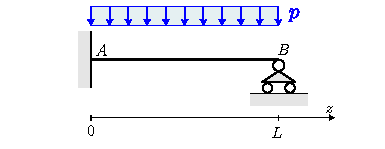
\includegraphics[scale=1.3]{figure/problema_elastico/iperstatica_LE}
\end{center}
\begin{svolgimento}
Osserviamo che nel punto $A$ sono assegnate tutte le componenti di spostamento generalizzato e dunque quel punto appartiene a $\partial_{D}\Lc$. Nel punto $B$, invece, è assegnata soltanto la componente verticale dello spostamento; in quel punto possiamo allora assegnare le forze generalizzate attive, ovvero una coppia e una forza orizzontale: in quel punto di frontiera ci sono condizioni al bordo \emph{miste}.

Scelta l'ascissa $z$ come in figura, il vincolo di incastro in $A$ richiede che siano soddisfatte le seguenti condizioni al bordo di natura cinematica:
\begin{equation}
v(0)=0, \qquad \varphi(0)=0 \quad \Longrightarrow \quad -v'(0)=0;
\end{equation}
analogamente, il carrello in $B$ richiede che
\begin{equation}
v(L)=0.
\end{equation}
Inoltre, l'assenza di coppie  in $B$ impone che
\begin{equation}
	M(L)=0 \quad \Longrightarrow \quad  v''(L)=0.
\end{equation}
Visto che la trave è puramente flessibile, la condizione $N(L)=0$ non è rilevante.
Dobbiamo dunque risolvere il seguente problema per determinare $v$:
\begin{equation}
	\begin{cases}
&v''''(z)=\dfrac{p}{EJ}\\[.2cm]
& v(0)=0\\
& v'(0)=0\\
& v(L)=0\\
& v''(L)=0.
\end{cases}
\end{equation}
Integrando in successione l'equazione differenziale, si ottiene:
\begin{equation}
v'''(z)=\frac{pz}{EJ}+a, \quad v''(z)=\frac{pz^2}{2EJ}+az+b, \quad v'(z)=\frac{pz^3}{6EJ}+a\frac{z^2}{2}+bz+c, \quad \frac{pz^4}{24EJ}+a\frac{z^3}{6}+b\frac{z^2}{2}+cz+d.
\end{equation}
Le 4 costanti di integrazione $a$, $b$, $c$, $d$ si determinano con le 4 condizioni al contorno. Dopo qualche calcolo, si ottiene
\begin{equation}
a=-\frac{5}{8} \frac{pL}{EJ}, \quad b=\frac{pL^2}{8EJ}, \quad c=d=0,
\end{equation}
da cui
\begin{equation}
	v(z)=\frac{pz^4}{24EJ}-\frac{5}{48}\frac{pL}{EJ}z^{3}+\frac{pL^{2}}{16EJ}z^{2}.
\end{equation}
Noto lo spostamento, possiamo determinare la curvatura
\begin{equation}
	\kappa(z)=- v''(z)=-\frac{pz^2}{2EJ}+\frac{5}{8EJ}\,pLz-\frac{pL^2}{8EJ},
\end{equation}
il momento flettente
\begin{equation}
M(z)=	EJ\kappa(z)=-\frac{pz^2}{2}+\frac{5}{8}\,pLz-\frac{pL^2}{8},
\end{equation} 
e il taglio, tramite l'equilibrio:
\begin{equation}
T(z)=M'(z)=-pz+\frac{5}{8}pL.
\end{equation}

Valutando le funzioni $T(z)$ e $M(z)$ al bordo, determiniamo il valore delle reazioni vincolari:
\begin{equation}
r_{A2}=T(0)=\frac{5}{8}pL, \quad c_{A}=M(0)=-\frac{pL^2}{8}, 	\quad r_{B2}=T(L)=-\frac 38 pL.
\end{equation}

Per comprendere il significato dei segni occorre fare riferimento alle convenzioni utilizzate nella Fig. \ref{fig:conciopiano}, che riportiamo sotto:
\begin{center}
		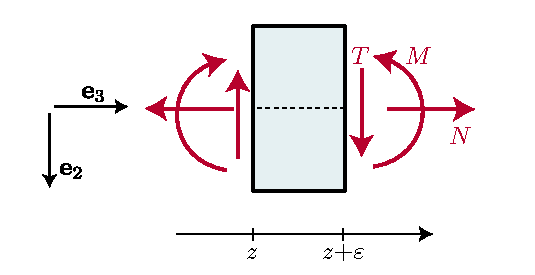
\includegraphics[width=0.5\linewidth]{figure/equilibrio/concio_piano}
\end{center}

Per il punto $A$ occorre vedere la faccia sinistra del concio. Il fatto che $T(0)$ sia positivo significa che in quel punto è presente una forza diretta verso l'alto; che $M(0)$ sia negativa significa che in quel punto c'è una coppia flettente antioraria, che tende dunque le fibre di sopra; infine, il taglio negativo in $B$ denuncia la presenza di una forza diretta verso l'alto. La situazione è quella riportata sotto. 
\begin{center}
	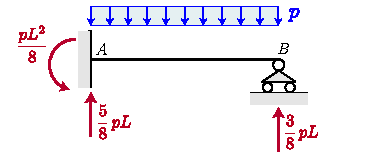
\includegraphics[scale=1.3]{figure/problema_elastico/iperstatica_LE1}
\end{center}
Rappresentiamo sotto i diagrammi delle caratteristiche della sollecitazione e la funzione $v(z)$, che fornisce la deformata della trave.
\begin{center}
	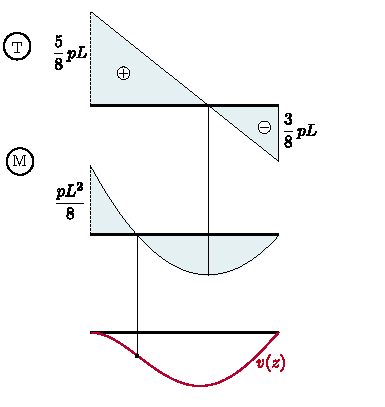
\includegraphics[scale=1.3]{figure/problema_elastico/iperstatica_LE2}
\end{center}
Osserviamo che dove $T$ è nullo, $M$ ha un punto stazionario; inoltre, dato che $M=-EJv''$, dove il momento si annulla, c'è un cambio di concavità della funzione $v(z)$.


\end{svolgimento}
\end{exercise}

\section{Formulazione in sforzi}
In questo approccio sono assunte come incognite primarie le caratteristiche della sollecitazione.
Se la struttura è isostatica, la formulazione è banale: si risolvono le equazioni di bilancio e si determinano le caratteristiche di sollecitazione; poi, tramite le equazioni costitutive si trovano le deformazioni e, infine, gli spostamenti integrando le equazioni di congruenza.

Se il sistema è iperstatico, le reazioni vincolari non sono determinabili in maniera univoca  con le sole condizioni di equilibrio e pertanto non si è direttamente in grado di trovare le caratteristiche della sollecitazione. Vediamo come procedere utilizzando il semplice esempio, che abbiamo già analizzato nella Sez. \ref{classif}.

\begin{center}
	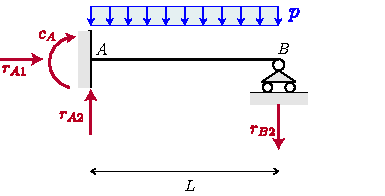
\includegraphics[scale=1.3]{figure/problema_elastico/iperstatica}
\end{center}

 Il sistema, che per semplicità assumiamo puramente flessibile,  è chiaramente iperstatico, con $\mathscr{i}=1$, ovvero è presente un vincolo sovrabbondante. Le equazioni di equilibrio
 \begin{equation}
 	\begin{cases}
 		r_{A1}=0,\\
 		r_{A2}-r_{B2}=p L,\\
 		-c_A-r_{B2}L=\frac{pL^2}{2},
 	\end{cases}
 \end{equation}
 ammettono una soluzione dipendente da un parametro, cui corrisponde una  un sistema di forze autoequilibrato:
 \begin{equation}\label{reazip}
 	r_{A1}=0, \qquad r_{A2}=pL+X, \qquad c_A=-\frac{p L^2}{2}-XL.
 \end{equation}
 Il parametro  $X\coloneqq r_{B2}$ prende il nome di \textit{incognita iperstatica}. Di conseguenza, le caratteristiche della sollecitazione dipendono da $X$:
 \begin{equation}\label{cdses}
N(z)=0, \qquad  T(z)=p(L-z)+X, \qquad M(z)=-\frac{pz^2}{2}+pLz-\frac{p L^2}{2}+X(z-L)
 \end{equation}
 avendo scelto un'ascissa con origine in $A$. A $M(z)$ corrisponde la deformazione
 \begin{equation}
 	\kappa(z)=\frac{M(z)}{EJ}=\frac{pz^2}{2EJ}+\frac{pLz}{EK}-\frac{p L^2}{2EJ}+\frac{X(z-L)}{EJ},
 \end{equation}
che, per essere congruente, deve rispettare la condizione
\begin{equation}\label{vsses}
\kappa(z)=-v''(z), \qquad \Longrightarrow \qquad -\frac{pz^2}{2EJ}-\frac{pLz}{EK}+\frac{p L^2}{2EJ}-\frac{X(z-L)}{EJ}=v''(z),
\end{equation}
con
\begin{equation}\label{bccongr}
v(0)=0, \qquad v'(0)=0, \qquad v(L)=0.
\end{equation}
Integrando la \eqref{vsses}, abbiamo
\begin{equation}
	v(z)=\frac{p}{24 EJ}(z^4-4L z+6L^2)+\frac{X}{6 EJ}(3L-z)z^2+c_1+c_2 z.
\end{equation}
La condizione $v(0)=0$ implica $c_1=0$, mentre  $v'(0)=0$ richiede che $c_2=0$. Resta da soddisfare l'ultima condizione:
\begin{equation}
v(L)=\frac{pL^2}{8EJ}+\frac{XL^3}{3EJ}=0
\end{equation} 
da cui si determina il valore dell'incognita iperstatica
\begin{equation}
X=-\frac{3}{8}\,pL.
\end{equation}
Dunque, tra le infinite caratteristiche della sollecitazione \eqref{cdses} equilibrate, parametrizzate da $X$, l'unica che risulta anche congruente è quella che corrisponde al valore dell'incognita iperstatica $X=-\frac{3}{8}\,pL$.
Dunque otteniamo
 \begin{equation}
	N(z)=0, \qquad  T(z)=\frac{5}{8}p L-pz, \qquad M(z)=-\frac p8 (L^2-5 L z+4 z^2),
\end{equation}
cui corrisponde la deformazione
\begin{equation}
	\kappa(z)=-\frac{p}{8EJ} (L^2-5 L z+4 z^2),
\end{equation}
e lo spostamento
\begin{equation}
v(z)=\frac{p}{24 EJ}\left(z^2-\frac{5}{2}z^3L+\frac{3}{2}z^2L^2  \right),
\end{equation}
concludendo così la soluzione del problema elastico.

Osserviamo che nelle reazioni vincolari \eqref{reazip}, così come in tutti i campi da quelle dedotti, si individuano due contributi
\begin{equation}
r_{A2}=r^{(0)}_{A2}+Xr^{(1)}_{A2}, \qquad c_A=c^{(0)}_A+Xc^{(1)}_A.
\end{equation}
Il primo contributo, indicato con l'apice $(0)$, è dovuto al carico esterno $p$ ed soluzione del problema di equilibrio in cui si ignora il vincolo in $B$, la cui reazione si è scelta come incognita iperstatica. Il secondo contributo,  indicato con l'apice $(1)$, è  dovuto ad una forza unitaria avente direzione e verso dell'incognita iperstatica scelta.

Osserviamo ancora che, delle tre condizioni al bordo \eqref{bccongr} relative alle equazioni di congruenza risulta rilevante solo la terza, quella che coinvolge lo spostamento in direzione e verso dell'incognita iperstatica. Le altre infatti, servono solo ad annullare lo spostamento rigido, impedito dalla presenza dell'incastro in $A$. Quindi, per determinare l'incognita iperstatica, di fatto è sufficiente trovare lo spostamento  del punto $B$ di applicazione dell'incognita iperstatica che ha chiaramente la rappresentazione
\begin{equation}
v_B=v_B^{(0)}+X\,v_B^{(1)},
\end{equation}
dove $v_B^{(0)}$ e $v_B^{(1)}$ rappresentano lo spostamento del punto di applicazione dell'incognita iperstatica, nella sua direzione e  verso, in due sistemi, in entrambi dei quali si è eliminato il vincolo corrispondente alla reazione $X$: nel primo si applica il carico reale e nel secondo una forza unitaria nella direzione e nel verso dell'incognita.

\begin{center}
	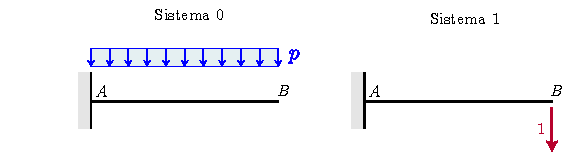
\includegraphics[scale=1.3]{figure/problema_elastico/iperstatica_sis}
\end{center}

Richiedendo che la condizione di vincolo reale sia soddisfatta, ovvero
\begin{equation}
v_B^{(0)}+X\,v_B^{(1)}=0,
\end{equation}
si determina l'incognita $X$, se si conoscono $v_B^{(0)}$ e $v_B^{(1)}$. Essendo tanto il sistema 0 quanto il sistema 1 isostatici, la determinazione dello spostamento del punto $B$, piuttosto che per integrazione dell'equazione di congruenza, può essere facilmente condotta facendo uso dell'equazione dei lavori virtuali, come descritto nella Sez. \ref{ELVimp}.

Per determinare lo spostamento $v_B^{(0)}$ dobbiamo dunque scegliere come sistema congruente il sistema 0, mente come sistema equilibrato il sistema 1. È immediato trovare che
\begin{equation}
M_0=-\frac{pz^2}{2}+pLz, \qquad \Longrightarrow \kappa_0=\frac{1}{EJ}\left(-\frac{pz^2}{2}+pLz\right),
\end{equation}
e
\begin{equation}
	M_1(z)=z-L.
\end{equation}
Usando l'equazione dei lavori virtuali, si trova allora
\begin{equation}
v_B^{(0)}=\int_0^L	M_1\kappa_0=\frac{pL^4}{8EJ}.
\end{equation}
Per determinare lo spostamento $v_B^{(01)}$ occorre scegliere sia come sistema congruente che equilbrato il sistema 0; si trova allora che
\begin{equation}
v_B^{(1)}=\int_0^L	M_1\kappa_1=\int_0^L	M_1\frac{M_1}{EJ}=\frac{L^3}{3EJ},
\end{equation}
da cui
\begin{equation}
X=-\frac{v_B^{(0)}}{v_B^{(1)}}=-\frac{3}{8}\,pL,
\end{equation}
come già determinato.

Alla luce di queste considerazioni, possiamo pensare di procedere in generale come segue.

Data una trave o un sistema di travi vincolati in modo iperstatico,
si individua un sistema \textit{principale} isostatico `sopprimendo' tanti vincoli
semplici quant'\`{e} il grado di iperstaticit\`{a} $\mathscr{i}$ del sistema.
Scelte quindi le incognite iperstatiche
$\{{X}_j\},\,(j=1,2,\ldots,J\equiv\mathscr{i})$, si definiscono il sistema $0$ caricando il sistema principale con i carichi reali e i sistemi $1, 2, \ldots, J$, ciascuno dei quali è costituito dal sistema principale caricato con una forza unitaria nella direzione e nel verso dell'incognita iperstatica $X_j$ agente nel punto di applicazione dell'incognita stessa.

Attraverso le equazioni di
equilibrio si calcola lo stato di sollecitazione  per ciascun sistema e lo stato di deformazione dei sistemi  $1, 2, \ldots, J$. Le  $J$ equazioni necessarie a selezionare l’unica soluzione equilibrata compatibile con la risposta linearmente elastica attribuita alla travature vengono scritte di solito nella notazione introdotta da \textit{H. M\"{u}ller-Breslau}:
\begin{definition}
	\begin{equation}\label{MB}
	\eta_j=\eta_{j0}+\sum_{k=1}^J\eta_{jk}X_k,\quad j=1,2,\ldots,J.
\end{equation}
\end{definition}

Nella \eqref{MB}, i termini $\eta_j$ sono noti, una volta formulato il problema di equilibrio che si intende risolvere; i termini $\eta_{j0}$ e i coefficienti $\eta_{jk}$ delle incognite iperstatiche prendono il nome di \textit{coefficienti di influenza}. L'interpretazione è la seguente:
\begin{itemize}
	\item $\eta_j$ rappresenta, nel sistema reale, lo spostamento generalizzato (assoluto o relativo) della sezione di applicazione dell’incognita iperstatica $X_j$, valutato nella direzione e nel verso di $X_j$ stessa;
	\item $\eta_{j0}$ ($j=1,2,\ldots,J$) rappresenta, nel sistema principale assoggettato al sistema di carichi esterni applicati alla struttura, lo spostamento generalizzato (assoluto o relativo) della sezione di applicazione dell’incognita iperstatica $X_j$, valutato nella direzione e nel verso di $X_j$ stessa;
	\item $\eta_{jk}$ ($j,k=1,2,\ldots,J$) rappresenta, nel sistema principale assoggettato al sistema di carichi di indice $k$, lo spostamento generalizzato (assoluto o relativo) della sezione di applicazione dell’incognita iperstatica $X_j$, valutato nella direzione e nel verso di $X_j$ stessa.
\end{itemize}

Per calcolare i coefficienti di influenza, ci si avvale dell’equazione dei lavori virtuali. In particolare
\begin{itemize}
	\item per valutare $\eta_{j0}$, si sceglie come sistema congruente di spostamenti e misure di deformazione quello relativo allo stato elastico indotto dal sistema di carichi esterni, che ha indice 0; come sistema equilibrato di forze e caratteristiche di sollecitazione quello relativo allo stato elastico di indice j:
	\begin{equation}
		1\cdot\eta_{j0}=\int_{\mathcal{L}}N_j\varepsilon_0+T_j\gamma_0+M_j\kappa_0;
	\end{equation}
\item per valutare  $\eta_{jk}$, si sceglie come sistema congruente di spostamenti e misure di deformazione quello relativo allo stato elastico indotto dal sistema di carichi di indice $k$; come sistema equilibrato di forze e caratteristiche di sollecitazione quello relativo allo stato elastico di indice $j$:
\begin{equation}
	1\cdot\eta_{jk}=\int_{\mathcal{L}}(N_j\varepsilon_k+T_j\gamma_k+M_j\kappa_k.
\end{equation}
\end{itemize}


\begin{exercise}
Si consideri la trave in figura. Determinare le reazioni vincolari e le caratteristiche della sollecitazione, nell'ipotesi che la trave sia puramente flessibile.
\begin{center}
	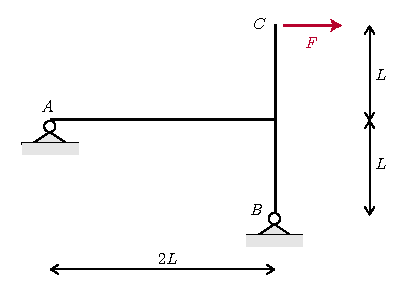
\includegraphics[scale=1.3]{figure/problema_elastico/iper_es1}
\end{center}

\begin{svolgimento}
Il sistema è composto da un singolo corpo e dunque $\mathscr{g}=3$; la molteplicità totale dei vincoli è $\mathscr{v}=2+2=4$ e dunque $\mathscr{g}-\mathscr{v}=-1=\mathscr{l}-\mathscr{i}$. Dato che evidentemente $\mathscr{l}=0$, essendoci due cerniere, concludiamo che $\mathscr{i}=1$ e dunque la struttura è una volta iperstatica. 
Scegliamo come unica incognita iperstatica la reazione orizzontale in $B$. Il sistema che si ottiene eliminando dunque il vincolo che esplica questa reazione, otteniamo una trave incernierata in $A$ e vincolata con un carrello ad asse verticale in $B$. Il sistema è chiaramente isostatico e dunque è un buon sistema principale. Costruiamo allora il sistema 0 e il sistema 1. 

\begin{center}
	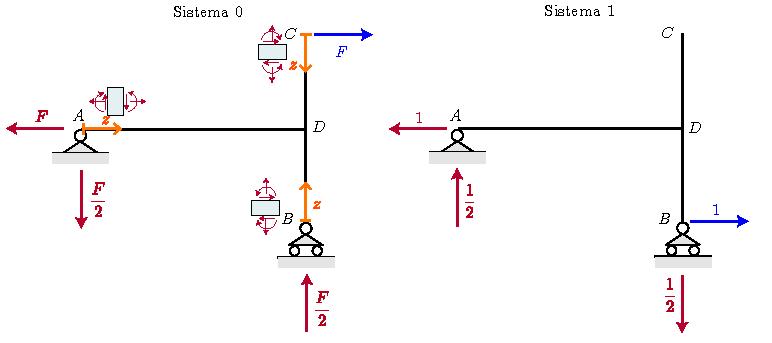
\includegraphics[scale=1.15]{figure/problema_elastico/iper_es1_1}
\end{center}

È immediato determinare le reazioni vincolari rappresentate in figura. I diagrammi del taglio e del momento flettente nel sistema 0 sono rappresentati sotto.

\begin{center}
	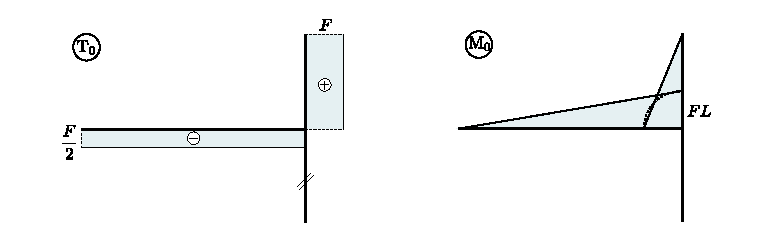
\includegraphics[scale=1.2]{figure/problema_elastico/iper_es1_2}
\end{center}

I diagrammi del taglio e del momento flettente nel sistema 1 sono rappresentati sotto.
\begin{center}
	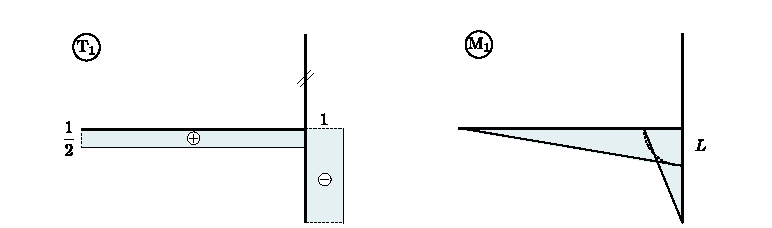
\includegraphics[scale=1.2]{figure/problema_elastico/iper_es1_3}
\end{center}

Utilizzando i sistemi di riferimento indicati in arancione in figura e le convenzioni dei segni dati dal concio infinitesimo ivi rappresentato, le funzioni rappresentative delle caratteristiche della sollecitazione su ogni tratto sono raccolte nella tabella sotto.

\vspace{.3cm}

\begin{tabular}{|c|c|c|c|c|}
	\hline
	Tratto & \(T_0\) & \(M_0\) & \(T_1\) & \(M_1\) \\ \hline
	$AD$ & \(-\dfrac{F}{2}\) & \(-\dfrac{F}{2}z\) & \(\dfrac{1}{2}\) & \(\dfrac{z}{2}\) \\[8pt] \hline
	$BD$ & 0 & 0 & $-1$ & $-z$ \\[8pt] \hline
	$CD$ & \(F\) & \(Fz\) & 0 & 0 \\[8pt] \hline
\end{tabular}

\vspace{.2cm}

Abbiamo adesso tutto il necessario per determinare i coefficienti dell'equazione di M\"uller-Breslau:
\begin{equation}
\eta_1=\eta_{10}+X\,\eta_{11}.
\end{equation}

La quantità $\eta_1$ rappresenta lo spostamento orizzontale del punto $B$ del sistema reale ed è dunque nullo, essendoci in quel punto una cerniera. Il coefficiente $\eta_{10}$ rappresenta lo spostamento orizzontale del punto $B$ nel sistema 0; può essere determinato usando l'equazione dei lavori virtuali:
\begin{equation}
\eta_{10}=\int_{\Lc}M_1 \kappa_0 =\int_{\Lc}M_1 \frac{M_0}{EJ}=\int_{0}^{2L}-\frac{Fz^2}{4EJ}=-\frac{2}{3}\frac{FL^3}{EJ}.
\end{equation}
il coefficiente $\eta_{11}$ rappresenta lo spostamento orizzontale del punto $B$ nel sistema 1; può essere determinato usando l'equazione dei lavori virtuali:
\begin{equation}
\eta_{11}=\int_{\Lc}M_1 \kappa_1=\int_{\Lc}\frac{M_1^2}{EJ}=\int_0^{2L}\frac{z^2}{4EJ}+\int_0^L\frac{z^2}{EJ}=\frac{L^3}{EJ}.
\end{equation}
Concludiamo che
\begin{equation}
X=-\frac{\eta_{10}}{\eta_{11}}=\frac{2}{3}P.
\end{equation}
Le caratteristiche della sollecitazione si possono trovare per sovrapposizione degli effetti. Sul tratto $AD$:
\begin{equation}
T=T_0+X T_1=-\frac{F}{6}, \qquad 
\end{equation}

\end{svolgimento}


\end{exercise}











